\documentclass[]{finalproject}
\usepackage[algoruled, linesnumbered, noline]{algorithm2e}
\usepackage{float}
\usepackage{graphicx}
\usepackage{minted}
\usepackage{ragged2e}
\graphicspath{{./img}}

\usepackage[parfill]{parskip}
\let\circledS\undefined % here - PS
\usepackage{amssymb}
\usepackage{enumitem}
\usepackage{caption}
\usepackage{mathtools}

\captionsetup{labelfont={bf}}

% Title (and subtitle) of the project
\title{Quicksort}
\subtitle{}

% Group members for the final project (comment out the unnecessary entries)
\begin{groupmembers}
\studentA{Pratyai}{}{Mazumder}
\studentB{Lodovico}{}{Mazzei}
\studentC{Michele}{}{Chersich}
\end{groupmembers}

\abstract {
  In this project, we examine Quicksort as a divide-and-conquer sorting algorithm.
  After presenting the algorithm and its design,
  we analyze its time complexity, as well as its scaling properties,
  in order to explain why it has become such a widely popular choice
  in computer science.
  We also introduce the problem domain of computational geometry,
  where the solutions to many problems can be seen as generalizations of Quicksort.
  Finally, as a practical application, we present the convex hull problem and the Quickhull algorithm,
  featuring analogous runtime and scaling properties.
}


\begin{document}
\maketitle

\section{Introduction} \label{introduction}

Sorting is a ubiquitous problem in computer science, with applications in practically every subfield
(e.g. data structures, computation geometry, search engines, etc.).

The sorting problem can be defined as the reordering of a sequence of elements, based on some ordering criterion.
More specifically, to be able to sort it, a sequence must possess following two 
properties\footnote{Either of these requirements can be relaxed for a relaxed variant of the sorting problem.}:

\begin{itemize}
\item Its elements are \textit{swappable}: So that the list can be permuted in-place\footnote{I.e. modifying the original sequence object, instead of creating a new one.}.
\item Any two of its elements are \textit{comparable}: i.e. the elements have total ordering \cite{towiki}.
\end{itemize}

Additionally, for many sorting algorithms, such as Quicksort, the sequence must also be \textit{randomly accessible}.

Many different algorithms were invented for the comparison sort problem. Quicksort, originally invented in 1962 by C. A. Hoare \cite{hoare1962quicksort}, is still one of the most commonly used sorting algorithms. The particularly interesting nature of Quicksort is that, unlike many other sorting algorithms, it does not even attempt to achieve the theoretical lower bound of worst-case complexity, i.e. $\Omega(n\log n)$ \cite[p.~193]{clrs}. Instead it has a fast average case and a much simpler implementation, making it a very practical choice.

There are many variants of the Quicksort algorithm, however, we will only focus on the worst-case and average-case analysis of one representative example.

\section{The algorithm}

\subsection{The partitioning problem}

Quicksort belongs to the family of \textit{partition sort} algorithms, where a partitioning routine is called recursively until the whole sequence is sorted.

Given an array $A[1,.....,N]$, the partitioning algorithm splits a permutation of it, $A'$, into two partitions $U=A'[1,.....,p]$ and $V=A'[p+1,.....,N]$
such that $U[i] \leq V[j] \;\, \forall \; i \in [1,p], j \in [p+1,N]$. By recursively partitioning U and V themselves, base cases will eventually be reached,
consisting of single-element or empty arrays, which are already sorted. Figure \ref{fig:rec-part} illustrates the recursive routine.

\begin{figure}[H]
\centering
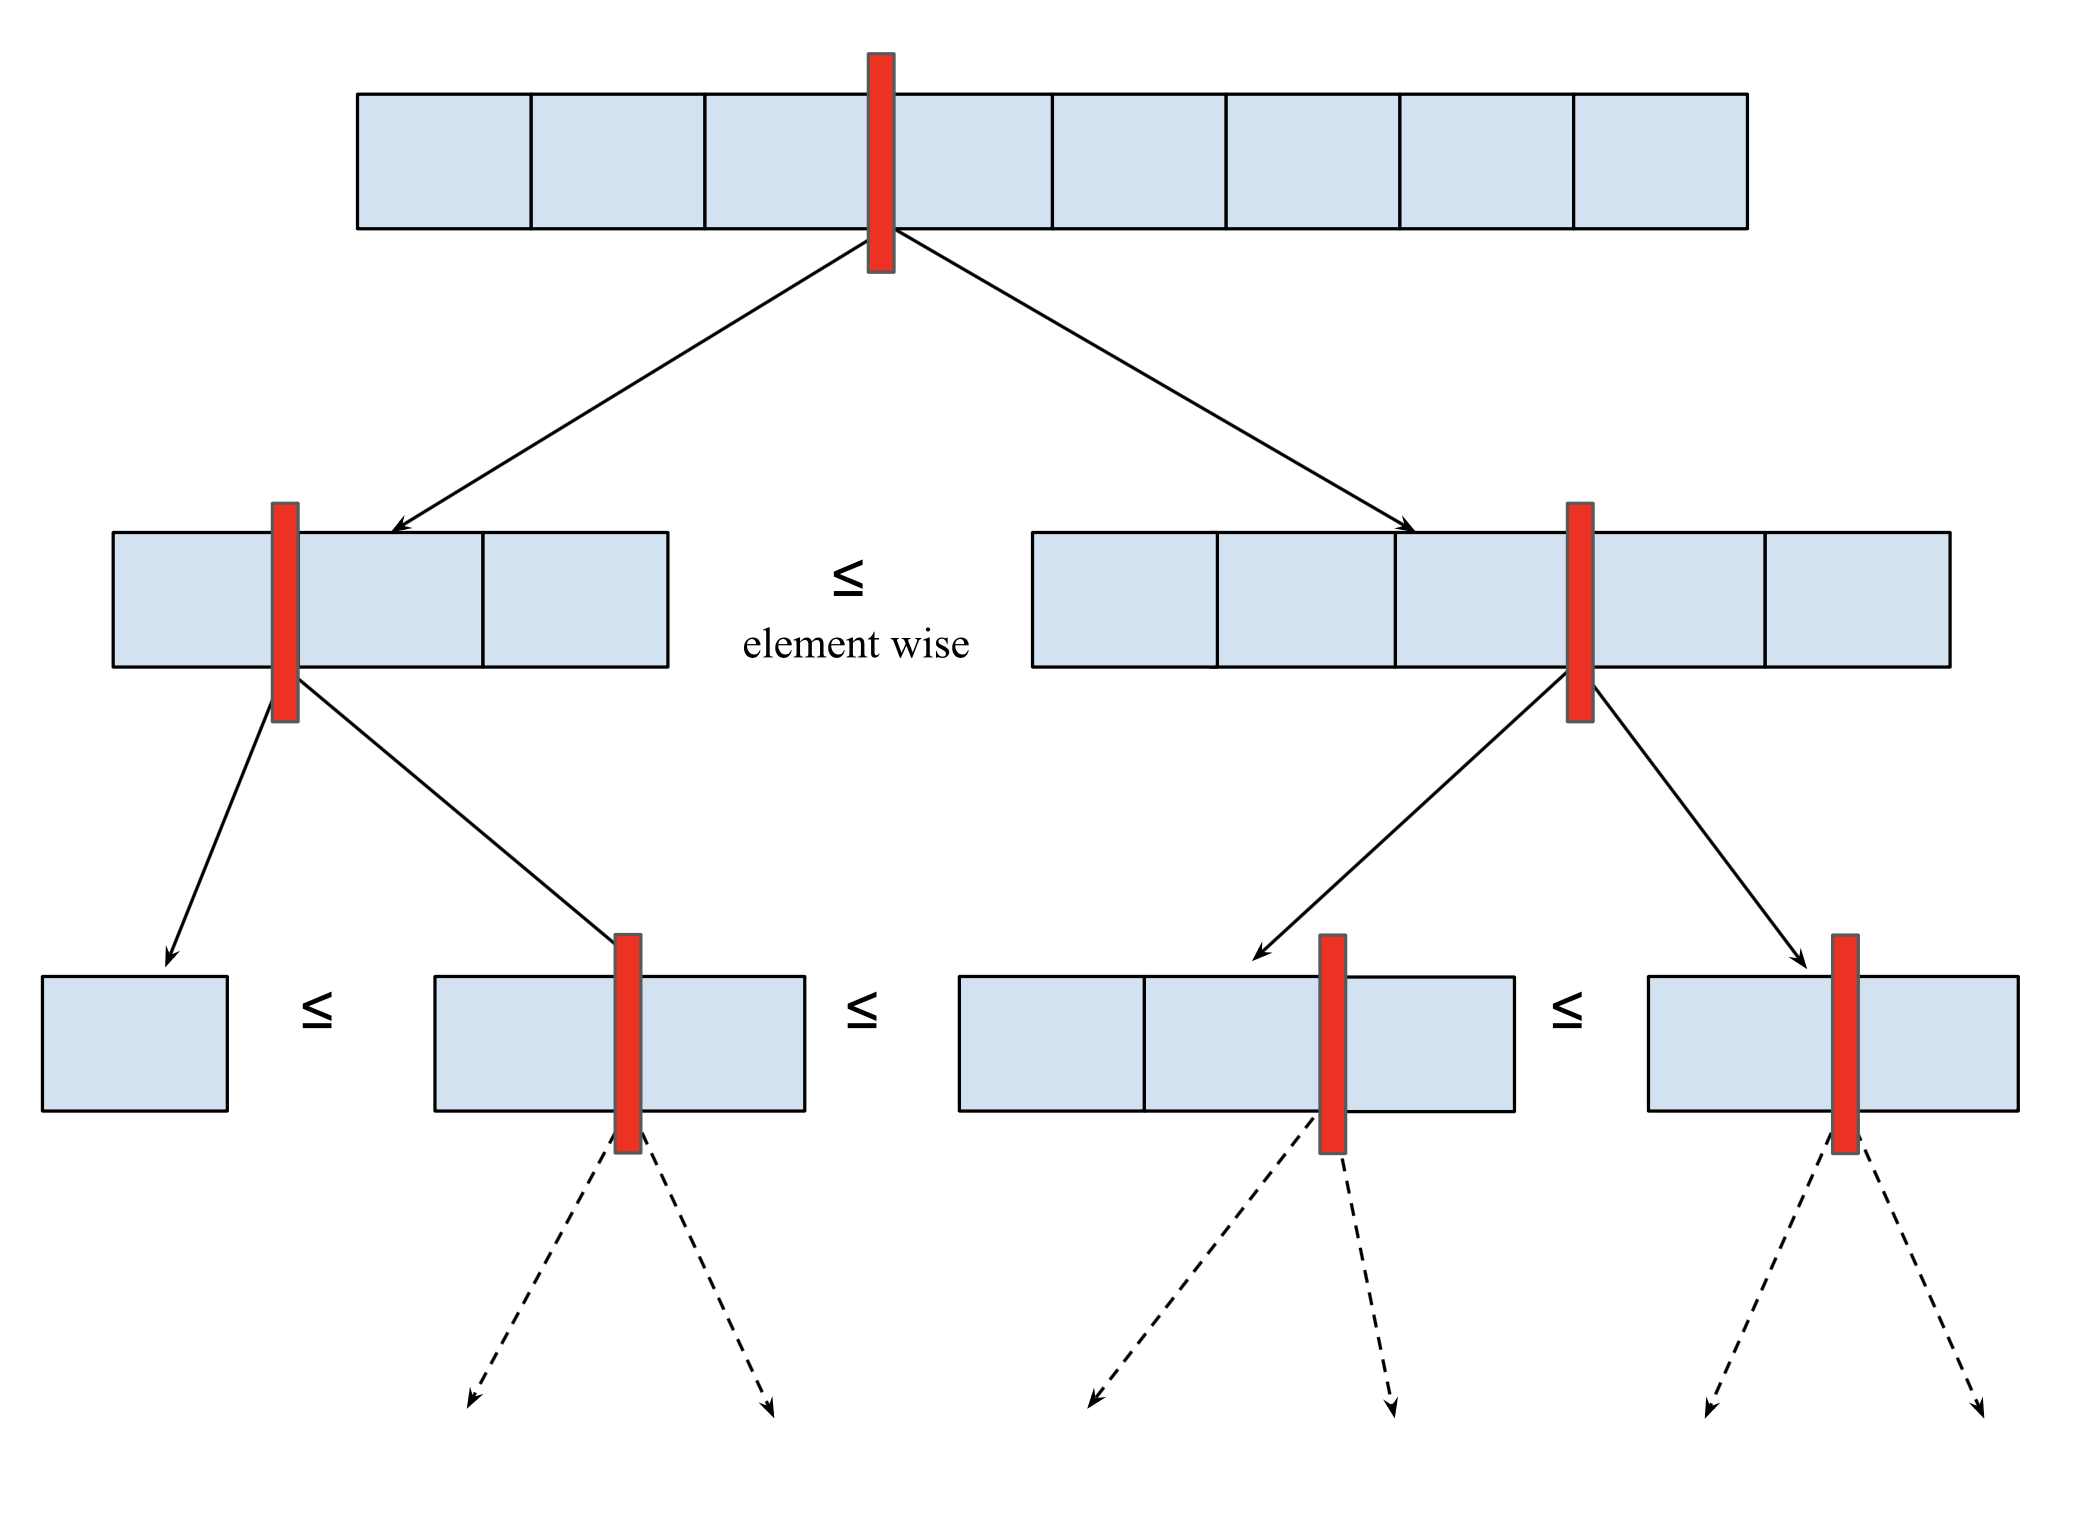
\includegraphics[width=0.5\textwidth]{recursive_partitioning.png}
\caption{Tree representation of the partitioning process.
At each level the array is permuted and split into two subarrays, where all elements in the left subarray are smaller than or equal to all elements in the right subarray.
The base case of a branch is reached when an array is reduced to one or zero elements.}
\label{fig:rec-part}
\end{figure}

The following pseudocode recursively sorts a given subarray of $A$.
It references a \texttt{partition} routine which will be discussed in the following sections.
Also, the \texttt{partition} routine will move one element (called \textit{pivot}) to its final location,
so that element can be excluded from the recursive calls.

\begin{algorithm}
\caption{Quicksort ($A$, $low$, $high$)}
\label{alg:p1}
\If(){$low \geq 0 ~\&\&~ high \geq 0 ~\&\&~ low < high$}{pivot := partition(A, low, high)\\
quicksort(A, low, pivot-1)\\
quicksort(A, pivot+1, high)}
\end{algorithm}

\subsection{Pivot selection}
The partitioning in Quicksort relies on pivoting. This consists in picking a value $\gamma$ to be our pivot.
Given an array $A$, we permute it such that every element before $\gamma$ is smaller than it, and every one after it is larger.
The internal order in these subarrays is irrelevant, as it will be addressed in further iterations of the algorithm.
Clearly, the pivot choice has an impact on the efficiency of the algorithm. We divide the selection methods into two categories: one-step and multi-step.
These are discussed using an example array $A[1, ..., N]$, as follows.

\subsubsection{One-step selection}
These methods only require choosing a single value at each iteration and using it as the pivot. Some examples are:

\begin{itemize}
\item \textit{First element}: select $A[1]$ as the pivot.
\item \textit{Last element}: select $A[N]$ as the pivot.
\item \textit{Central element}: letting $k=\frac{N+1}{2}$, select $A[floor(k)]$ or $A[ceil(k)]$ as the pivot.
\item \textit{Random element}: select $A[r]$ as the pivot, where $r$ is a random number such that $1 \leq r \leq N$.
\end{itemize}

\subsubsection{Multi-step selection}
Given that the best partitioning is achieved when picking the median of some array sample of size T, where T is an odd number, typically $3 \leq T \leq 9$.

\begin{itemize}
\item \textit{Median-of-T with fixed selection}: $T$ integers $1 \leq n_{1},....,n_{T} \leq N$ are fixed beforehand. \\
The median of $\{A[n_{1}],.....,A[n_{T}]\}$ is used as the pivot.
\item \textit{Median-of-T with random selection}: $T$ random integers $1 \leq r_{1},....,r_{T} \leq N$ are generated. \\
The median of $\{A[r_{1}],.....,A[r_{T}]\}$ is used as the pivot.
\end{itemize}

\subsection{Partitioning around the pivot}
There are several schemes to partition a list around the pivot. Two common choices are the Hoare scheme and the Lomuto scheme \cite{qs-scheme}.
For the purpose of this project, we will focus on the former.

Figure \ref{fig:rec-part2} illustrates the process of partitioning around a pivot. We start with two iterators \texttt{i} and \texttt{j},
initialized at offsets $0$ and $N+1$ respectively, and move the iterators towards each other while maintaining the conditions \texttt{A[i] < pivot}
and \texttt{A[j] $\geq$ pivot}. When both iterators fail their conditions, we swap \texttt{A[i]} and \texttt{A[j]}.
When \texttt{i} and \texttt{j} meet, the partitioning step is complete. This process is defined in Algorithm \ref{alg:p2}.

\begin{algorithm}
\caption{partition($A$, $low$, $high$)}
\label{alg:p2}

pivot = selectPivot(A)

i, j := low - 1, high + 1

loop forever

\Indp

do i := i + 1 while $A[i] < pivot$

do j := j - 1 while $A[j] \geq pivot$

\If(){$i \geq j$}{return}

swap A[i] with A[j]
\end{algorithm}

\begin{figure}[H]
\begin{center}
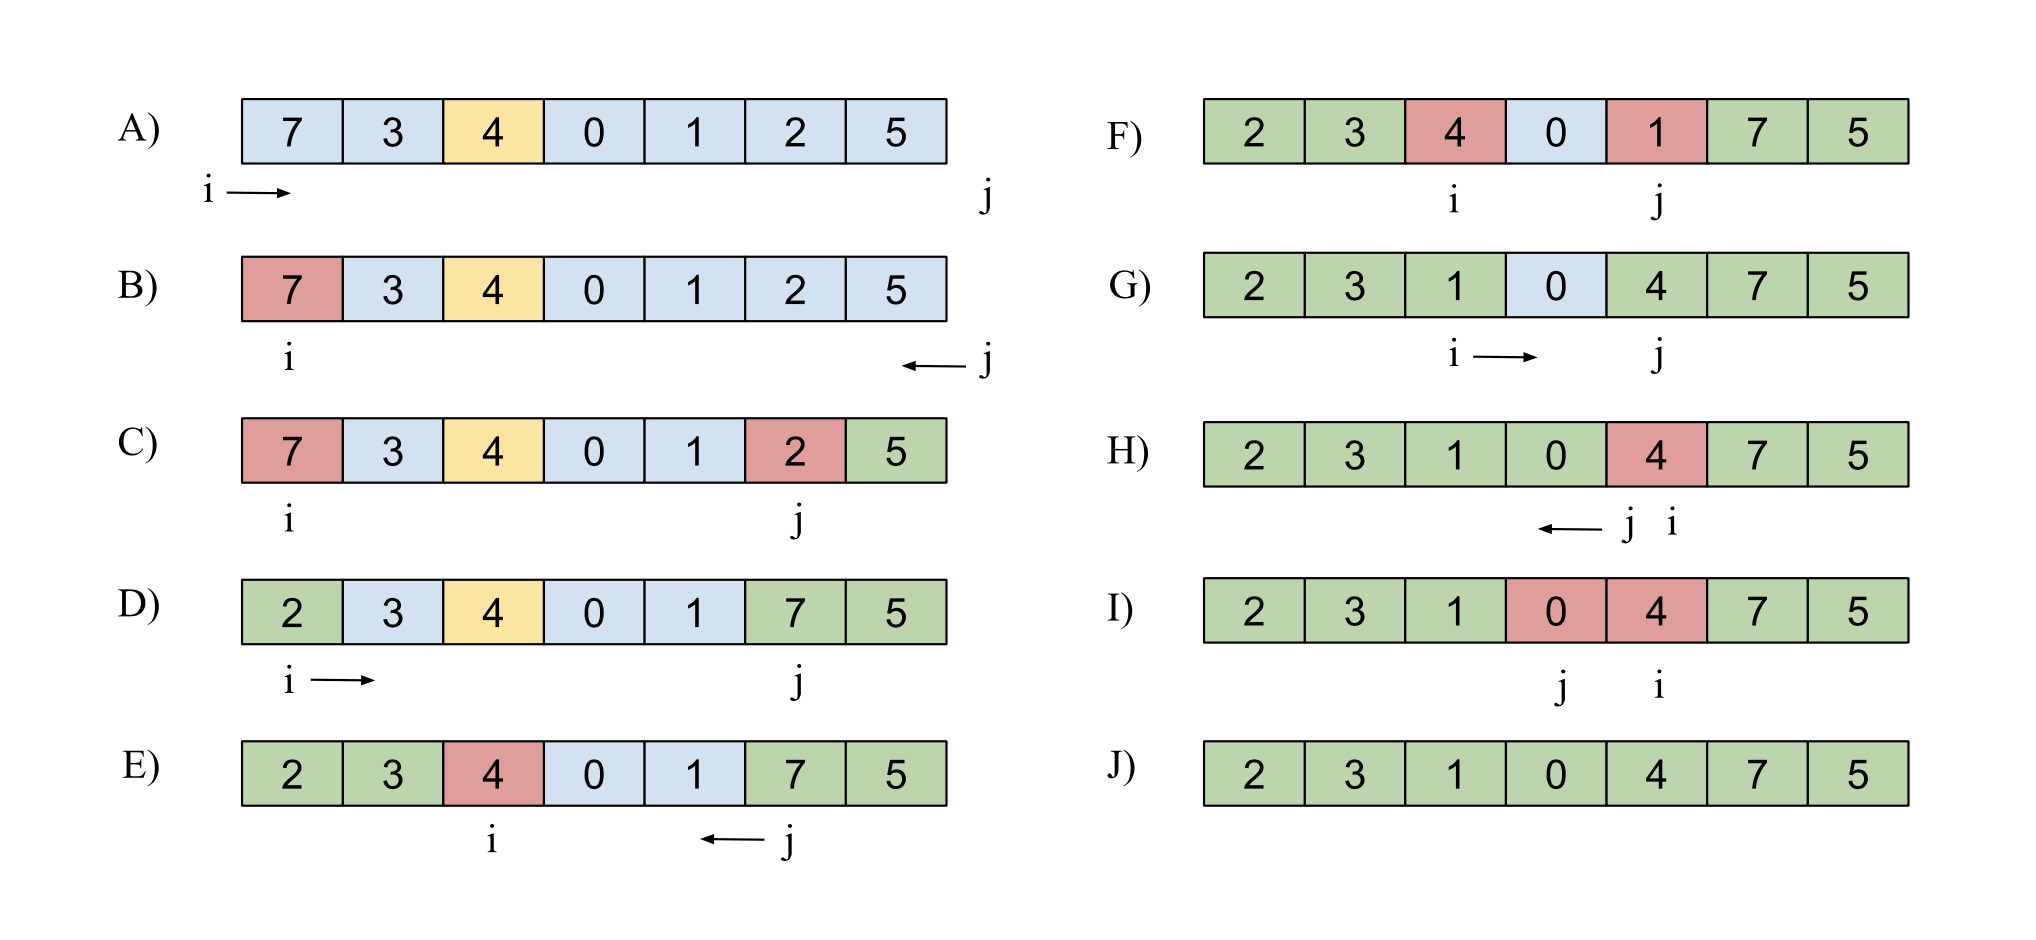
\includegraphics[scale=0.4]{img/pivot_partitioning.png}
\end{center}
\caption{Partitioning of the array around the pivot $p=4$ (yellow).
Blue elements are yet to be checked; red elements need to be swapped; green elements are already in the correct partition.\\
\textbf{A-B-C)} Start with $i$ at position $0$ and $j$ at position $N+1$: $i$ stops at $7$, $j$ stops at $2$: $i<j$, so $A[i]$ and $A[j]$ are swapped.
\textbf{D-E-F)} $i$ next stops at $4$, $j$ stops at $1$: $i<j$, so $A[i]$ and $A[j]$ are swapped.
\textbf{G-H-I)} $i$ and $j$ move until they cross.
\textbf{J)} End of iteration: all elements to the right of the pivot 4 are greater or equal than it, and all the ones to its left are smaller.}
\label{fig:rec-part2}
\end{figure}


\section{Complexity analysis}

We will consider the notion of algorithm complexity to be the growth of its computational cost with respect to some input parameters.
In general the cost can be any runtime resources the algorithm needs.
Here, we will restrict the analysis to an estimation of how fast the computation time grows with the size of the input sequence.

We will also assume an extremely simplified model of execution that does not consider cache, locality of reference, hardware architecture, etc.,
all of which have significant impact on computation time. In this model, the only expensive operations are comparison and swap,
each costing $\Theta({1})$.
Everything else, including the recursive function calls and random number generations, is negligible.

\subsection{Analysis of \texttt{partition} routine}

Let's consider the Hoare scheme outlined in Algorithm \ref{alg:p2}. The first operation is the selection of the pivot,
which is $\Theta(1)$ for all selection methods mentioned above.

Once the pivot is selected, we scan the subarray in $n = high - low + 1$ steps, each involving exactly one comparison between the current pointees,
one occasional comparison between the pointers themselves, and one occasional swap between the current pointees.
So, each step is $\Theta(1)$, and the total complexity of the \texttt{partition} routine is: $$T_{partition}(n) = \Theta(1) + n\Theta(1) \approx \Theta(n)$$
This complexity estimation holds true for all the pivot selection and partitioning schemes we have discussed, and also for any input data.

\subsection{Analysis of \texttt{quicksort} routine}

Now, let's consider the recursive \texttt{quicksort} routine outlined in Algorithm \ref{alg:p1}.
The first operation is a comparison to check the base case, which requires no additional computation.
Otherwise, we incur into exactly one call to the \texttt{partition} routine and two calls to the \texttt{quicksort} routine with the two partitions.
If the two partitions have sizes $u$ and $n-u-1$, the complexity of the \texttt{quicksort} routine is:
$$T(n) = T_{partition}(n) + T(u) + T(n-u-1) = T(u) + T(n-u-1) + \Theta(n)$$
This is a recursive formula where the partition sizes, $u$ and $n-u-1$, depend on the input data and the pivot selection method.
So, in order to get an explicit formula without recursion, we need to consider different input and pivot scenarios.
We will do this for the following two important cases, which are also the most typical for complexity analysis.

\subsubsection{Worst-case analysis}

The worst case for the \texttt{quicksort} routine occurs when the partitions are the least balanced,
i.e. the pivot element ends up being the largest or the smallest in the subarray. Therefore,
\begin{align*}
T_{worst}(0) &= \Theta(1) \\
T_{worst}(1) &= \Theta(1) \\
T_{worst}(n) &= T_{worst}(n-1) + T_{worst}(0) + \Theta(n) \\
\shortintertext{Expanding this recurrence until the base case, we find}
T_{worst}(n) &= \sum_{k=1}^n\Theta(k) = \Theta(n^2)
\end{align*}

\subsubsection{Average-case analysis}

For deterministic pivot selection methods, there is always some hostile input data for which the algorithm will meet the worst case.
However, in practical scenarios, running into hostile input data is fairly unlikely.
Instead, we are often interested in the average case analysis, that accounts for the prior distribution of the input data to compute the average cost.

Since the locations of the pivots determine the runtime of Quicksort for a given input data, and there is no other information about the pivot,
we will consider the prior distribution of the pivot location at each call to the \texttt{quicksort} routine to be uniform,
i.e. if the size of the given array is $n$, then its final location can be anywhere between and including 1 and n. So, the average sorting time will be
\begin{align*}
T(n) &= \frac{1}{n}\sum_{k=1}^{n}\big(T(k-1) + T(n-k)\big) + \Theta(n) \\
&= \frac{1}{n}\big(\sum_{k=1}^{n}T(k-1) + \sum_{k=1}^{n}T(k-1)\big) + \Theta(n) \\
&= \frac{2}{n}\sum_{k=0}^{n-1}T(k) + cn ~~~~~[\text{for some constant $c$}]\\
nT(n) &= 2\sum_{k=0}^{n-1}T(k) + cn^2 \\
nT(n) - (n-1)T(n-1) &= 2T(n-1) + 2cn - c \\
\implies nT(n) &\approx (n+1)T(n-1) + 2cn \\
\shortintertext{From this recurrence we get the set of equations}
\frac{T(n)}{n+1} &= \frac{T(n-1)}{n} + \frac{2c}{n+1} \\
\frac{T(n-1)}{n} &= \frac{T(n-2)}{n-1} + \frac{2c}{n} \\
&~~\vdots \\
\frac{T(2)}{3} &= \frac{T(1)}{2} + \frac{2c}{3} \\
\shortintertext{Adding them up yields}
\frac{T(n)}{n+1} =  \frac{T(1)}{2} + 2c \sum_{k=3}^{n+1}\frac{1}{k} &= \frac{T(1)}{2} + 2c\Big(\log(n+1) + \gamma - \frac{3}{2}\Big) ~~~~~[\text{$\gamma \approx 0.577$ is the Euler's constant}] \\
\implies T(n) &= O(n\log n)
\end{align*}

\subsection{Analysis of randomized Quicksort}

Instead of deterministic pivots, we can also select a random element from the subarray, with uniform probability.
This way we obtain the exact same analysis of the average case and the complexity order $O(n\log n)$. However, there are a few notable distinctions:
\begin{itemize}
\item Our execution model ignores the cost of random number generation (RNG).
With randomized pivots, we generate $O(n\log n)$ random numbers, which can have substantial impact, depending on the RNG implementation.
\item With deterministic pivot selection, there is always some hostile permutation of the input array for which the algorithm will degenerate to the worst case.
With randomized pivots, for any input data the expectation is the average case.
Theoretically, the RNG can still select a pivot on the boundary everytime.
However, it is extremely unlikely in practice for any decent RNG implementation and a reasonably large array.
\end{itemize}

\section{Parallelizing Quicksort}

Quicksort is fairly simple to parallelize, with a few modifications. Here we present a distributed approach, called \textit{sample sorting}.
The algorithm starts with the input sequence of size $n$, evenly distributed over $p$ processors, connected by some network.
Every processor holds a partition of roughly $\frac{n}{p}$ size.
The procedure of the distributed version of Quicksort is given in Algorithm \ref{alg:qs-dist}.

\begin{algorithm}
  \caption{Distributed Quicksort}
  \label{alg:qs-dist}
  Each processor selects $s$ randomly sampled elements as candidate pivots from the data it holds, and sends them to the \textit{manager} processor.

  The manager processor sorts the candidate pivots locally and select $p-1$ evenly spaced pivots, and sends the selected pivots to every worker processor.

  Every processor locally $p$-partitions its own data using the $p-1$ pivots received from the manager processor.
  It may happen that some partitions turn out empty this way.

  Every processor sends its local $k$-th partition to the $k$-th processor in the network.

  Every processor collects all the local partitions it received and sorts them locally,
  resulting in a distributed sorted permutation of the original input sequence.
\end{algorithm}

\begin{figure}[H]
\centering
\begin{minipage}{.49\linewidth}
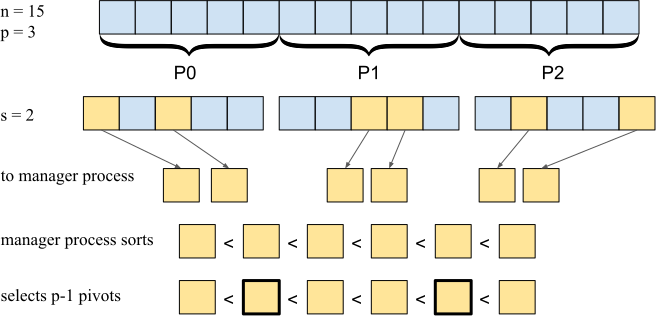
\includegraphics[width=\linewidth]{par-qs-1.png}
\end{minipage}
\begin{minipage}{.49\linewidth}
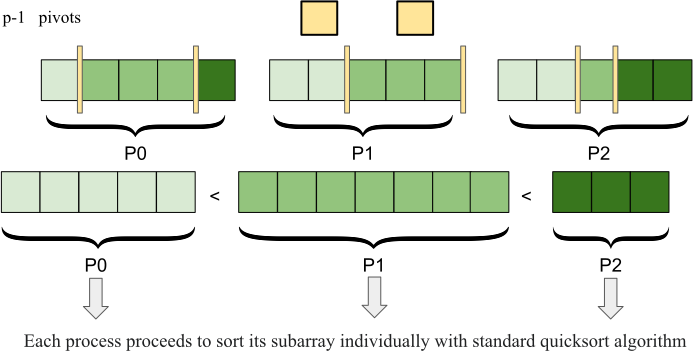
\includegraphics[width=\linewidth]{par-qs-2.png}
\end{minipage}
\caption{Distributed sample sorting: in the pivot selection process (left), each processor selects 2 candidate pivots (yellow) from the local data, then the manager process sorts all the candidate pivots to pick 2 pivots (yellow with thick border). All of the selected pivots are passed to each processor (right), which $p$-partitions the data with these pivots (the partions are highlighted in shades of green) and send each partition to the appropriate processor. Finally each processor locally sorts the accumulated partitions.}
\label{fig:par-qs}
\end{figure}

The challenges of such distributed sorting algorithms are about optimizing inter-processor communication, which usually cost much more than local operations.

\section{Computational geometry and the convex hull problem}
Computational geometry is the study of algorithms for the solution of geometric problems in the Euclidean space \cite{jaja2000perspective}.
The convex hull problem belongs to this class of problems, and has a wide range of applications across several disciplines
(e.g. data classification, collision avoidance, image processing and recognition). It is defined as follows:
given a set of points, find the smallest convex polygon containing all the points \cite{geowiki}.
For the purpose of this project, we will consider only the planar convex hull, with 2D Cartesian coordinates.

\subsection{The Quickhull algorithm}
The Quickhull algorithm is a variation of Quicksort for the solution of the convex hull problem.
The algorithms works as follows:
an initial partitioning step is done by picking the leftmost and rightmost points.
Let these two points be respectively $p_1$ and $p_2$.
The line connecting $p_1$ and $p_2$ splits the set in two parts.
For each subset, we search for the farthest point from the line: let this point be $p_{max}$.
If it exists, the points lying inside the triangle $p_1p_2p_{max}$ are removed from the set,
and the recursive step is applied on the points that lie outside the lines $p_1p_{max}$ and $p_2p_{max}$.
Again, let $p_1$ and $p_2$ be the end points of the line in the recursive step.
The stop condition occurs when $p_{max}$ does not exist, as there are no points outside $p_1p_2$.
The very first steps of the algorithm are illustrated in Figure \ref{fig:qh-steps}.
The pseudocode is given in Algorithms \ref{alg:qh1} and \ref{alg:qh2}.

\begin{figure}[H]
    \centering
    \begin{minipage}{.245\linewidth}
		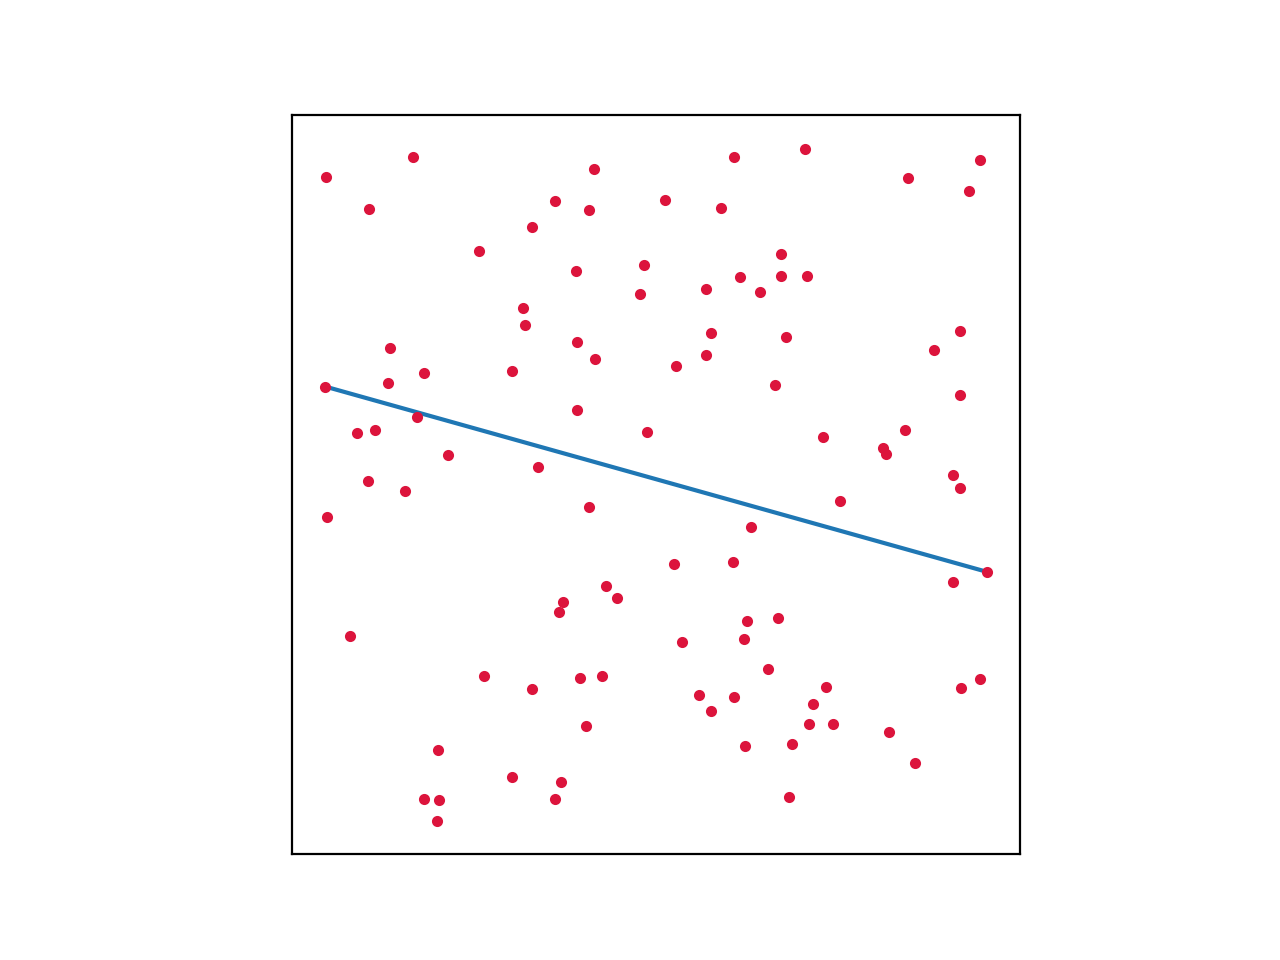
\includegraphics[width=\linewidth]{quickhull1.png}
	\end{minipage}
	\begin{minipage}{.245\linewidth}
		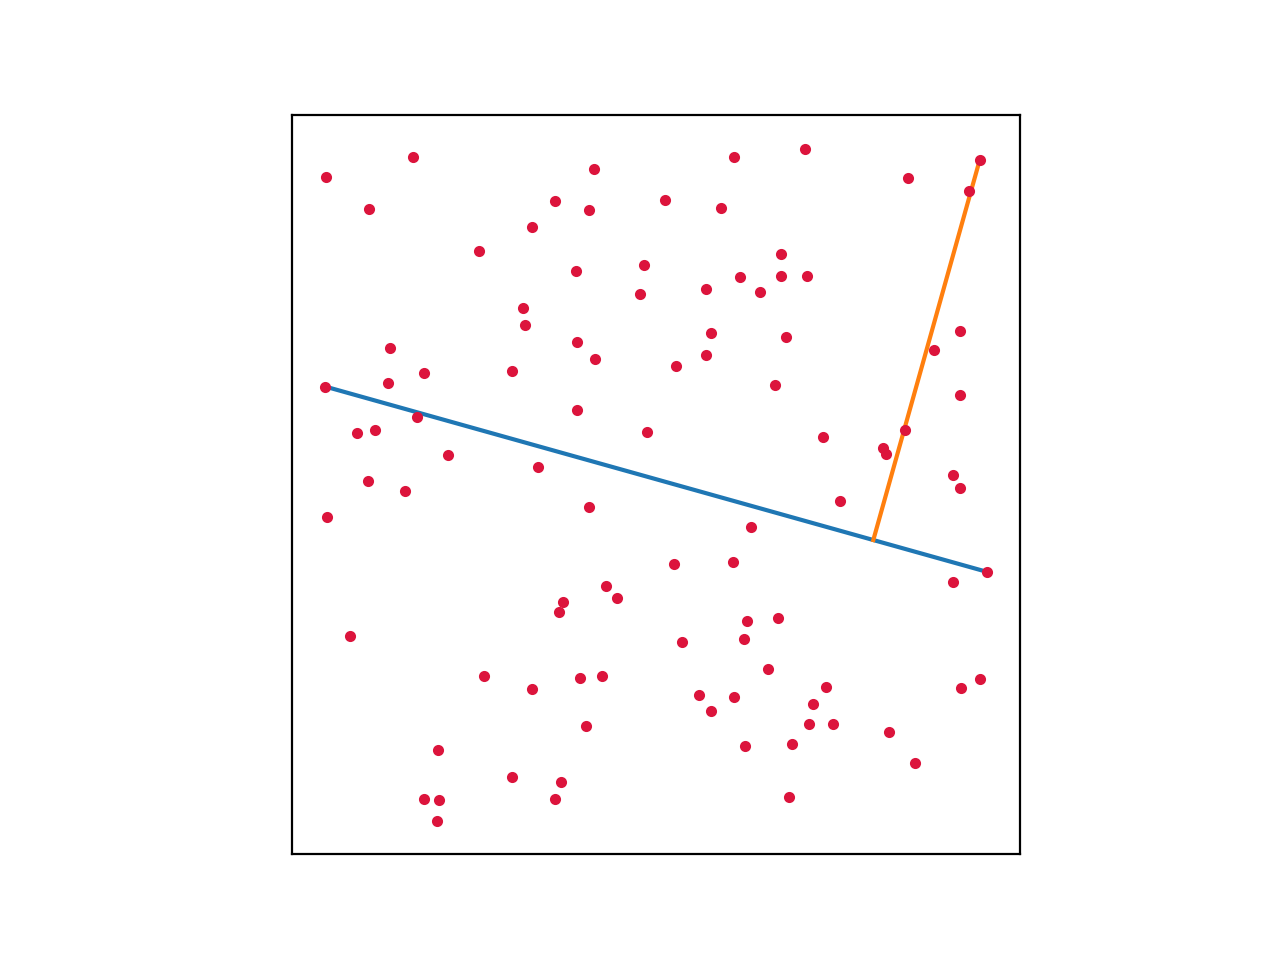
\includegraphics[width=\linewidth]{quickhull2.png}
	\end{minipage}
  \begin{minipage}{.245\linewidth}
		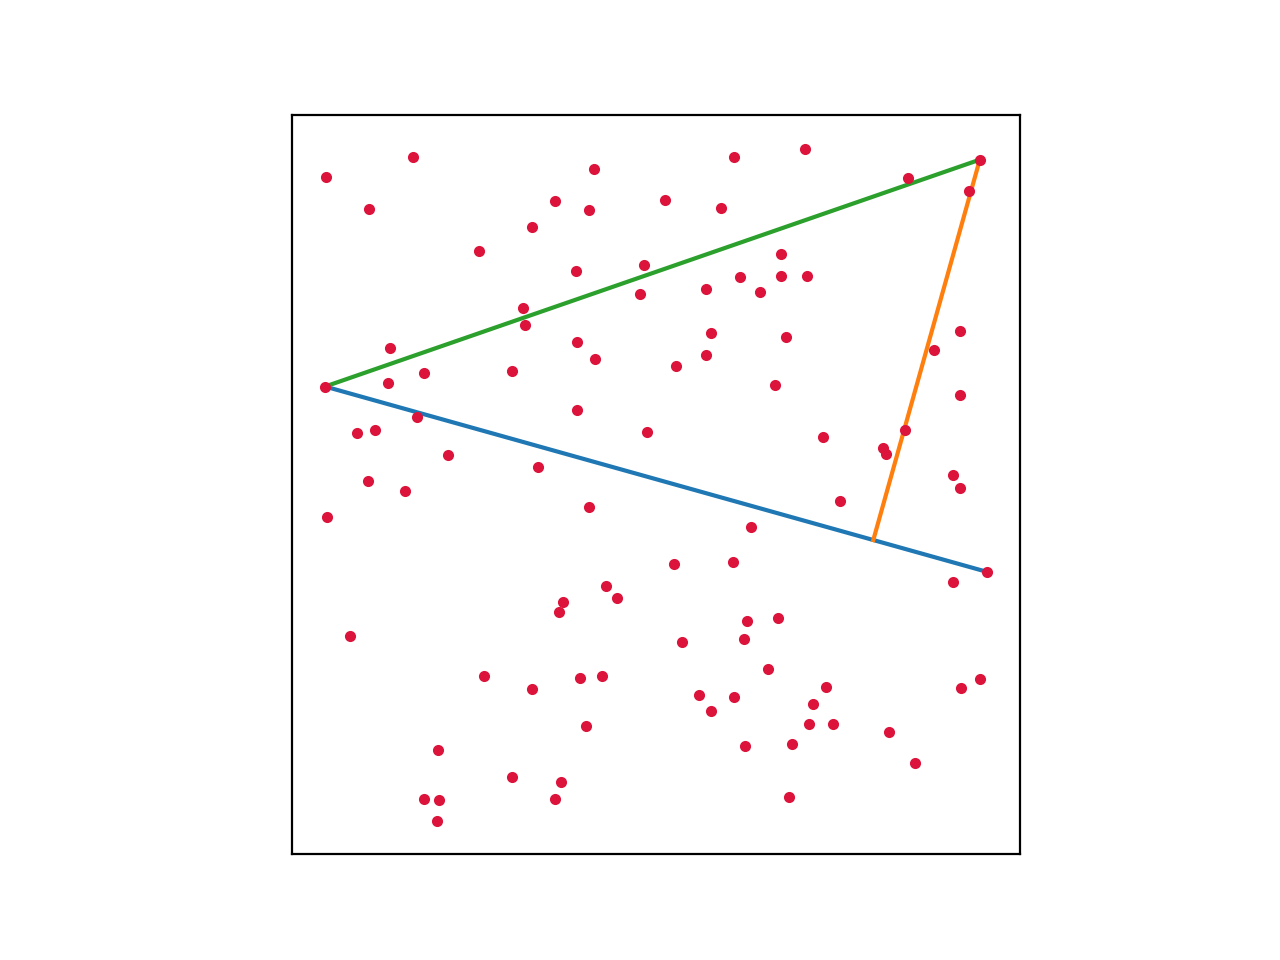
\includegraphics[width=\linewidth]{quickhull3.png}
	\end{minipage}
  \begin{minipage}{.245\linewidth}
		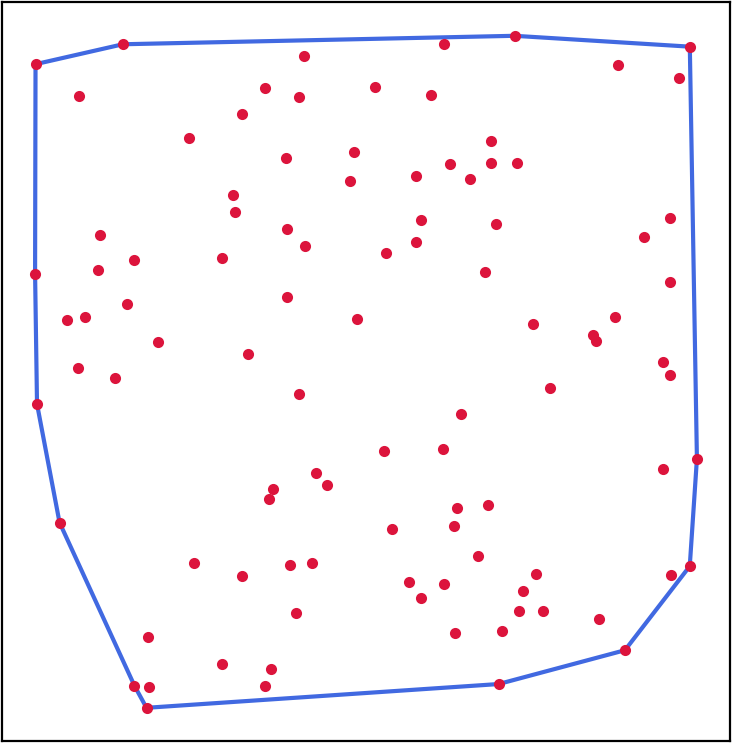
\includegraphics[width=\linewidth]{quickhull4.png}
	\end{minipage}
    \caption{Three steps of the Quickhull algorithm: the line $p_1p_2$ partitions the set of points in two subsets (1); the farthest point $p_{max}$ from the line is found (2); the recursive step considers just the outer points for the solution (3); at the end, the point set P is just the convex hull (4).}
    \label{fig:qh-steps}
\end{figure}

\begin{algorithm}
    \caption{Quickhull ($P$)}
    \label{alg:qh1}
    P is a set of points with coordinates (x, y)

    Find the points $p_1$ and $p_2$ with x-coordinates $x_{min}$ and $x_{max}$

    Quickhull\_onside($P$, $p_1$, $p_2$, $1$)

    Quickhull\_onside($P$, $p_1$, $p_2$, $-1$)
\end{algorithm}
\begin{algorithm}
  \caption{Quickhull\_onside ($P$, $p_1$, $p_2$, $s$)}
  \label{alg:qh2}
  Let $p_{max}$ be the the point that is farthest from the line $p_1p_2$, on side $s$

  \If(){$p_{max}$ does not exist}{return}

  Remove from $P$ all points that lie in the triangle $p_1p_2p_{max}$

  Let $s_1$ and $s_2$ be the outer sides of lines $p_1p_{max}$ and $p_2p_{max}$

  Quickhull\_onside($P$, $p_{max}$, $p_1$, $s_1$)

  Quickhull\_onside($P$, $p_{max}$, $p_2$, $s_2$)
\end{algorithm}

We can observe how Quickhull, just like Quicksort,
is both a divide-and-conquer and a sorting algorithm. The former approach is implemented by partitioning,
splitting the initial problem into smaller subproblems in a recursive fashion, whereas the latter is applied by comparing
Euclidean distances between points. Again, the complexity is $O(n^2)$ in the worst case and $O(n\log{n})$ in the average case.

\subsection{Distributed Quickhull}
The Quickhull algorithm is sequential by design,
as each recursive call depends on the previous ones for the computation of the solution set \cite{rameshconvex}.
Therefore, parallelizing the algorithm by multithreading is not feasible, as it is not possible to independently compute the solution to subproblems.
However, the set of points can be distributed over multiple processes, and inter-process communication can be used to combine the partial results.\\
The procedure of the distributed version of Quickhull is given in Algorithm \ref{alg:qh3}.

\begin{algorithm}
  \caption{Distributed Quickhull ($P$)}
  \label{alg:qh3}
  Each process computes the points with minimum and maximum x-coordinate among their local dataset, then the global minimum and maximum are computed, and broadcast to all processes (\textit{allreduce}).

  Each process computes the farthest point from the line joining the two points, and the global result is found (\textit{allreduce}).

  Once each process has all three vertices of the triangle, they can remove the points that lie inside the triangle from their dataset.

  The recursive step is repeated just like in the sequential version.

  At the end, the solution is scattered over all processes, so it must be gathered on the root process (\textit{gather}).
\end{algorithm}

The procedure is almost identical to the sequential version.
The key difference is the use of inter-process communication in the partitioning steps:
the computation performed by each process to find the leftmost and rightmost points, as well as the farthest point at every iteration,
is limited to a subset of points, so the results of all processes must be combined, in order to obtain the global result.
Note that communication is used just for the aforementioned purpose, and to combine the final solution on the root process,
keeping the communication cost low.

\subsubsection{Scaling analysis}
Running the algorithm for large input sizes with different numbers of processes, we can observe significant gains in performance.
A scaling chart is reported in Figure \ref{fig:qh-scaling}.
\begin{figure}[H]
\centering
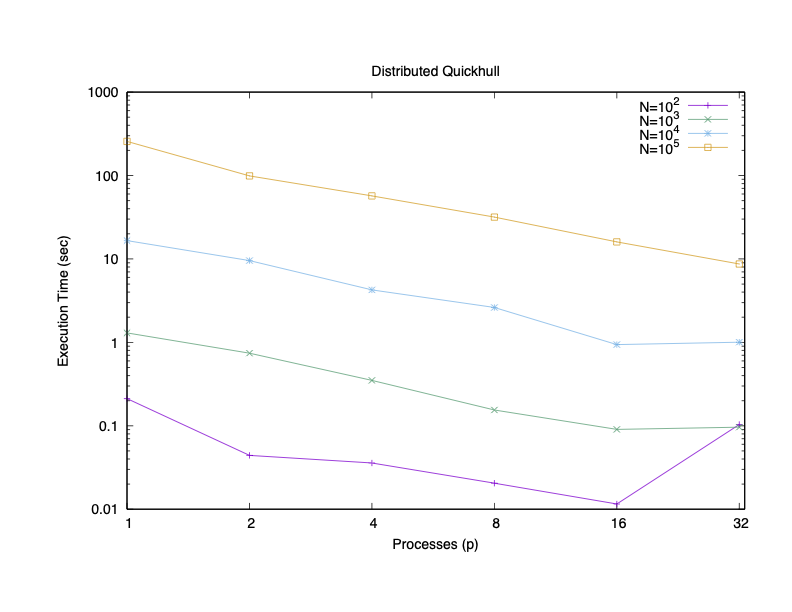
\includegraphics[width=0.5\linewidth]{gpStrongTime.png}
\caption{Performance scaling of distributed Quickhull.}
\label{fig:qh-scaling}
\end{figure}

We can observe the gain in performance obtained by the distributed version of the algorithm:
by doubling the number of processes, the execution time decrease by a factor 2, if the problem size is large enough (e.g. $N=10^5$).
However, for small problem sizes, we can observe the effect of over-parallelizing,
as the execution time decreases by smaller and smaller factors, or does not decrease at all
(e.g. for $N=10^2$, 32 processes perform worse than 16).

\section{Conclusion}
We analysed the Quicksort algorithm as a divide-and-conquer sorting algorithm. Its simplicity, as well as its appealing average-case runtime,
make it a very popular choice among known sorting algorithms. Furthermore, its scaling properties allow to exploit distributed
systems for significant gains in performance. By analysing the Quickhull algorithm in computational geometry,
we have shown an example of how the design principles of Quicksort can be generalized and applied to different problem domains.

%%%%%
\clearpage
\bibliographystyle{abbrv}
\bibliography{references}



\end{document}
